\thispagestyle{plain}
\mbox{}
\vspace{2in}
\begin{center}
{\em ``Give orange me give eat orange me eat orange give me eat \\ orange give me you.''} \\ [2ex]				
\hfill
% \footnotesize{Longest recorded quotation from}
\footnotesize{---Nim Chimpsky}\footnote{
\leavevmode\vspace*{-\baselineskip}
\InsertBoxL{0}{\qquad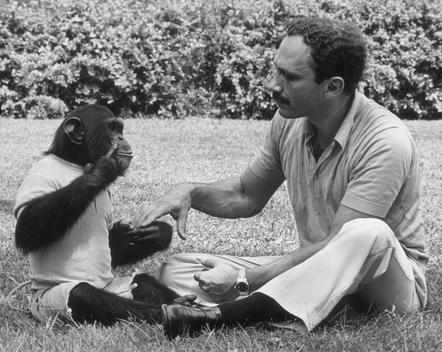
\includegraphics[height=2.7cm]{01-introduction/figs_and_tables/nim.jpg}}%
\vspace{7pt}
\noindent Nim Chimpsky (November 19, 1973 – March 10, 2000) was a chimpanzee who was the subject of an extended study of animal language acquisition at Columbia University, led by Herbert S. Terrace, as a challenge to Chomsky's thesis that full-fledged language use was innate only to humans. This quote is the Nim's longest recorded sentence.
 %, when translated from sign language
 }
\end{center}


\afterpage{\blankpage}


